\documentclass{article}

% if you need to pass options to natbib, use, e.g.:
%     \PassOptionsToPackage{numbers, compress}{natbib}
% before loading neurips_2018

% ready for submission
% \usepackage{neurips_2018}

% to compile a preprint version, e.g., for submission to arXiv, add add the
% [preprint] option:
%     \usepackage[preprint]{neurips_2018}

% to compile a camera-ready version, add the [final] option, e.g.:
     \usepackage[final]{neurips_2018}

% to avoid loading the natbib package, add option nonatbib:
\usepackage[nonatbib]{neurips_2018}
\usepackage[utf8]{inputenc} % allow utf-8 input
\usepackage[T1]{fontenc}    % use 8-bit T1 fonts
\usepackage{hyperref}       % hyperlinks
\usepackage{url}            % simple URL typesetting
\usepackage{booktabs}       % professional-quality tables
\usepackage{amsfonts}       % blackboard math symbols
\usepackage{nicefrac}       % compact symbols for 1/2, etc.
\usepackage{microtype}      % microtypography
\usepackage{graphicx}
\usepackage{float}
\usepackage{longtable}
\usepackage{multirow}
\usepackage{array}
\usepackage{tabularx}
\usepackage{diagbox}
\newcolumntype{n}{>{\arraybackslash}m{5.3cm}}
\newcolumntype{d}{>{\arraybackslash}m{8cm}}

\title{A data-driven study of physiotherapy for cystic fibrosis: identifying sub-types of airway clearance techniques and physical activity patterns using unsupervised clustering}

% The \author macro works with any number of authors. There are two commands
% used to separate the names and addresses of multiple authors: \And and \AND.
%
% Using \And between authors leaves it to LaTeX to determine where to break the
% lines. Using \AND forces a line break at that point. So, if LaTeX puts 3 of 4
% authors names on the first line, and the last on the second line, try using
% \AND instead of \And before the third author name.

%\author{%
%  David S.~Hippocampus\thanks{Use footnote for providing further information
%    about author (webpage, alternative address)---\emph{not} for acknowledging
%    funding agencies.} \\
%    I think we need to keep anonymous for our submission\\
%  Department of Computer Science\\
%  Cranberry-Lemon University\\
%  Pittsburgh, PA 15213 \\
%  \texttt{hippo@cs.cranberry-lemon.edu} \\
  % examples of more authors
  % \And
  % Coauthor \\
  % Affiliation \\
  % Address \\
  % \texttt{email} \\
  % \AND
  % Coauthor \\
  % Affiliation \\
  % Address \\
  % \texttt{email} \\
  % \And
  % Coauthor \\
  % Affiliation \\
  % Address \\
  % \texttt{email} \\
  % \And
  % Coauthor \\
  % Affiliation \\
  % Address \\
  % \texttt{email} \\
%}

\begin{document}


\maketitle

\begin{abstract}
  Children and young people with cystic fibrosis (CYPwCF) are prescribed physiotherapy including daily airway clearance techniques (ACT), and being physically active as part of their treatment. Little is known about how CYPwCF follow this advice in their everyday lives. Physiotherapy has evolved over the decades without the clarity of evidence that would accrue from detailed data. Such data are now being collected as part of Project [Anonymous] which is the largest CF physiotherapy trial in the UK to date. The data we analyse come firstly from novel pressure sensors attached to existing ACT devices which measure breathing patterns during normal treatments, and secondly from Fitbit activity trackers which monitor physical activity patterns, from 139 participants over 9 months. In close collaboration with clinical experts, we quantified and characterised this unique ACT and activity data by creating custom features from the waveforms. Using unsupervised learning techniques, we identified meaningful sub-types, with k-means clustering achieving the best performance. We found 4 clusters of ACT data which were sensitive enough to track interventions in ACT routines. Within physical activity data we identified 4 clusters related to daily footsteps and 5 clusters related to heart rate data.
\end{abstract}

\section{Problem overview}

Cystic Fibrosis (CF) is the most common life-limiting inherited disorder in the UK. It is a genetic disorder that mainly affects the respiratory system. In the lungs, excessive thick sticky mucus can cause lung damage leading to a deterioration in health. Despite improvements in care, CF remains progressive and incurable. 

To promote clearance of mucus from the lungs, daily physiotherapy called airway clearance techniques (ACT) is prescribed \cite{Daniels2017}. ACT commonly involve around 10 sets of 10 exhalation breaths into an ACT device, once to twice per day. Some CYPwCF report that ACT is the most burdensome part of having the disease \cite{JamesLindAlliance}. Physiotherapists also encourage children to have a physically active lifestyle, which has been shown to reduce the rate of decline in lung function \cite{Williams2014}. Adherence to physiotherapy has traditionally been assessed via questionnaire or self report, both of which are known to be inaccurate. More objective measures of adherence have not been widely available, and the evolution of CF physiotherapy has not been informed by this important evidence \cite{Modi2006}.  

Previously, bespoke pressure sensors were developed which attach to existing ACT devices in order to facilitate remote monitoring of ACT undertaken routinely at home (recording pressure values in time-stamped millibars, sampling frequency 10~Hz) \cite{Zhang}. Previously, bespoke games were also developed which could be driven by pressure changes from breathing through the sensor. These are now being used in a study of 145 CYPwCF \cite{HelenDouglas2018} to quantify routine ACTs (using the pressure sensors) and physical activity patterns (using Fitbit activity trackers), and to study the effects of gamification. This is the largest CF physiotherapy trial in the UK, collecting completely novel daily data about how children follow physiotherapy advice in their everyday lives. The broader goals of the study are to link physiotherapy adherence patterns with clinical outcomes (like lung function) in order to optimise and personalise treatment, which could reduce treatment burden and improve patient outcomes. In this paper we describe the challenge of i) quantifying ACT pressure sensor data and Fitbit activity data by creating custom features of the waveforms (featurising), and ii) discovering sub-types of ACT and physical activity patterns using clustering techniques. These daily sub-types can be tracked over time, as interventions such as gaming are introduced.  
 
\section{Methods}

\subsection{Study design and analysis approach}

The 18 month study \cite{HelenDouglas2018} includes the following interventions: introducing feedback to participants on their ACTs (number of breaths per treatment) via a computer tablet application, introducing games, and later removing these interventions. The data presented here is from the first 9 months of the trial with 139 participants enrolled at staggered times. Participants ranged in age from 6-16 years old, came from 3 London hospitals, all consented to participate in the study, and all data were completely de-identified for analysis.
 
Our analysis seeks to find patterns in physiotherapy data, and as such, the data is unlabelled and we use an unsupervised learning approach. Unsupervised clustering has been shown to be a useful technique for analysis of healthcare data, including finding novel sub-types in physical activity data from wearables \cite{physical_activity_patterns_2017} and sub-types in a variety of diseases including arthtritis \cite{Eng2019} and sepsis \cite{Seymour2019}. A high-scale data analysis and exploration pipeline was built in R in a secure analysis environment.  

\subsection{Collaboration, trust and interpretability}

Many applications of machine learning to medical data fail to explain how (if at all) the expertise of clinicians has been included \cite{Alaa2018}. To address the issues that arise from a lack of collaboration \cite{Vayena2018}, \cite{Challen231}, \cite{Char2018}, \cite{Ahmad2018} our methodology involved close collaboration between data scientists and CF experts, making every data decision jointly. We used a novel approach of involving at least one clinical expert in engineering “stand-ups” every day over the course of building the data analysis pipeline (7 months). We only considered features that were meaningful to clinicians, and we balanced traditional statistical evaluation metrics, with what was interpretable to clinicians.  

\section{Experiments and results}

\subsection{Quantifying physiotherapy data and creating clinical features}

\subsubsection{Featurising ACT data}

Several pre-processing steps were performed on the raw pressure data which were a function of the custom sensor used, including assembling data packets and removing duplicate values. The sensor also introduced significant non-linear baseline drift, which was removed with a sparsity-based de-noising approach with an asymmetry factor, called BEADS \cite{Ning2014}. An example of pre-processing raw pressure data is shown in figure \ref{fig: Waveforms}.

\begin{figure}[htb]
  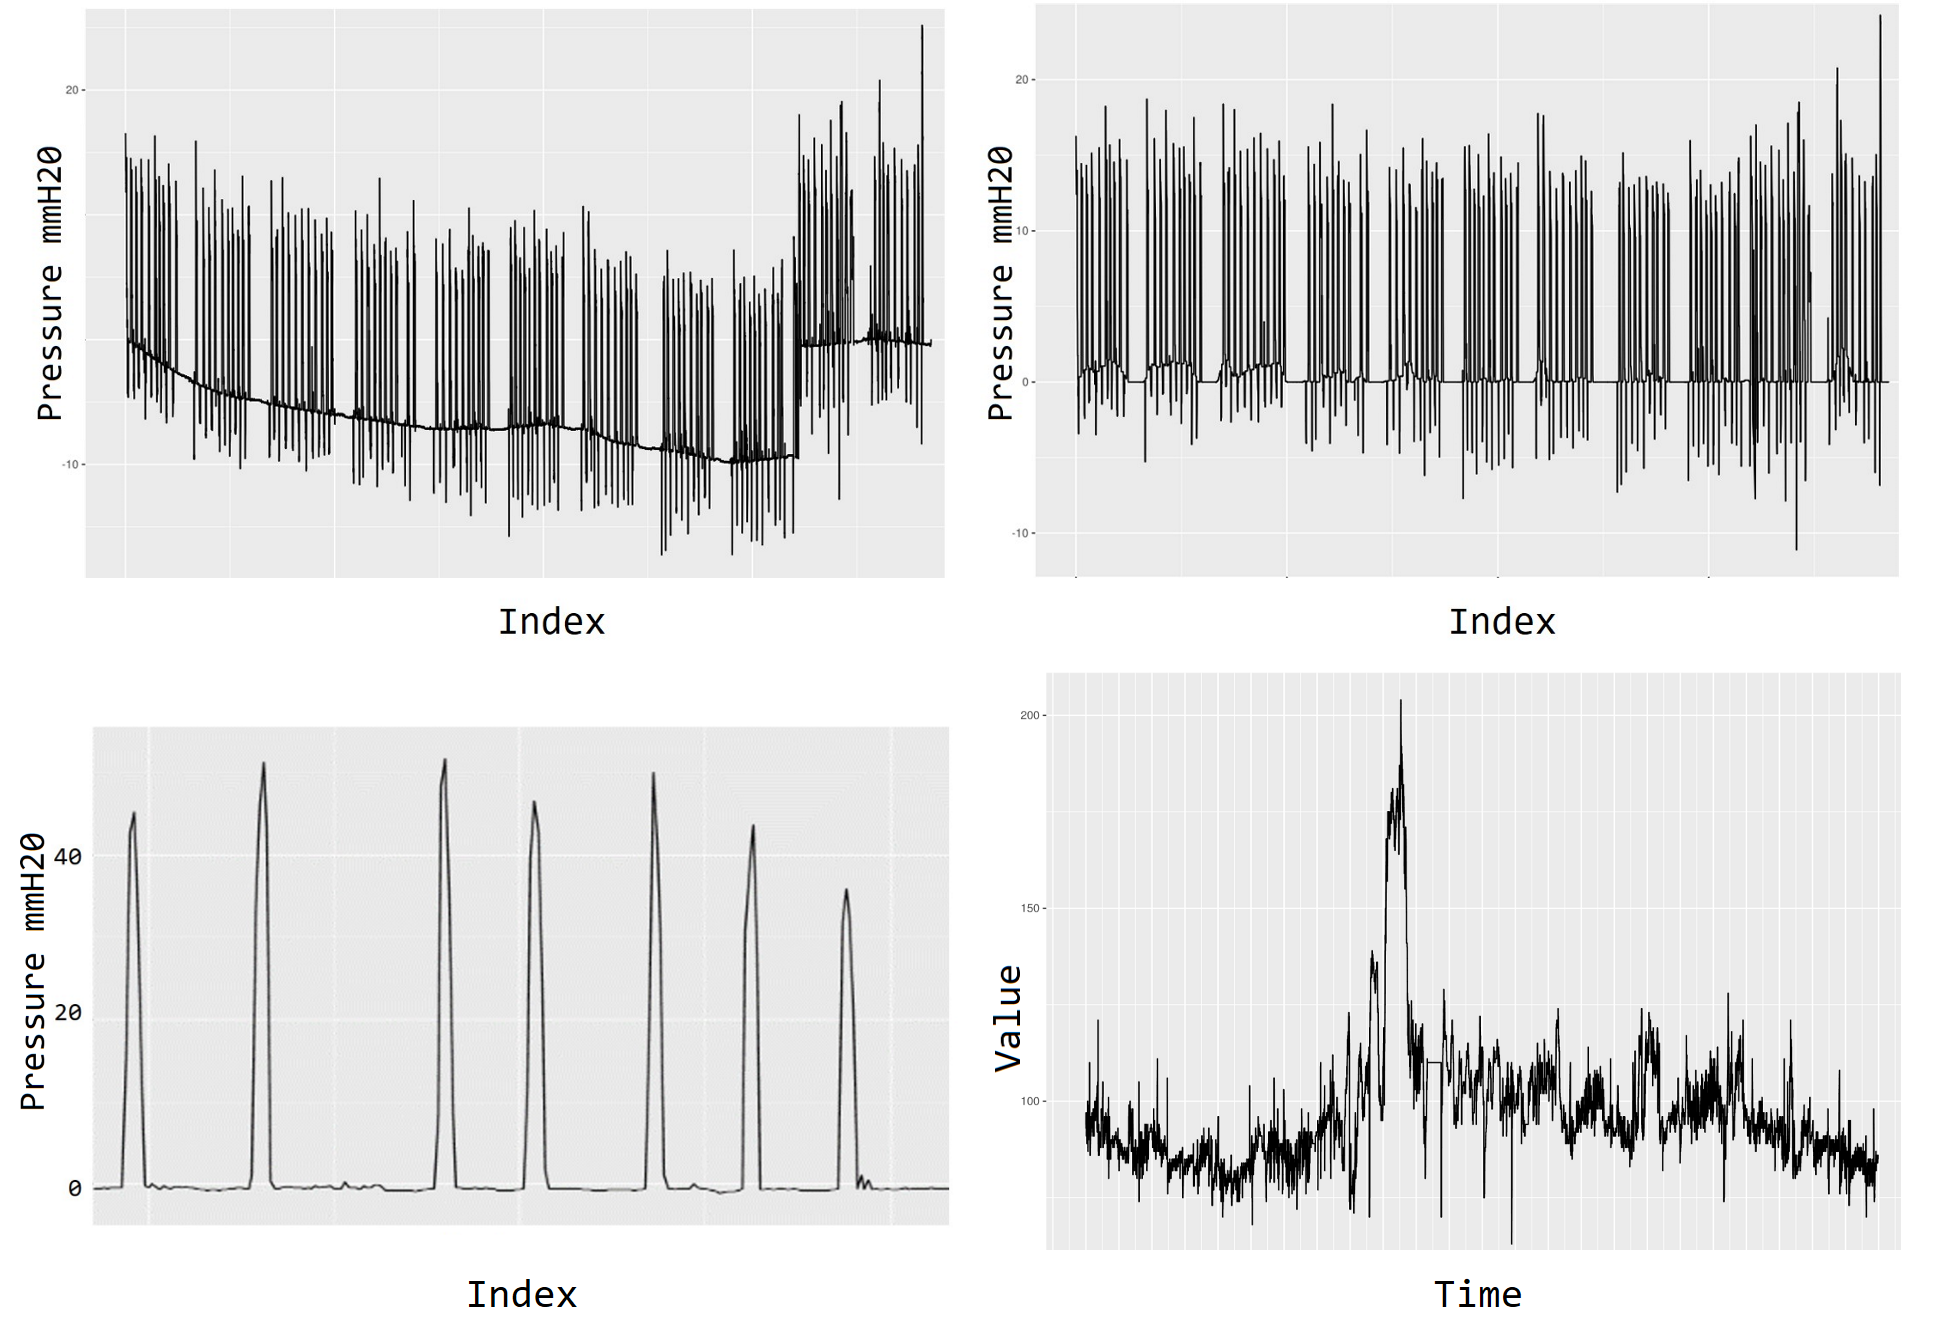
\includegraphics[width=\textwidth]{Waveforms.png}
  \centering
   \caption{Top left: raw ACT data in two packets, with baseline drift. Top right: Data packets assembled into a treatment and baseline drift removed. This treatment shows 11 sets of 10 exhalations (the positive peaks), lasting 33 minutes. Bottom left: A typical, pre-processed ACT waveform. This treatment is 20 seconds long and contains 7 exhalation breaths. Bottom right: One day showing heartrate data from the Fitbit with a sustained period of heartrate in MVPA.}
  \label{fig: Waveforms}
\end{figure}

In total, we recorded 24,434 sensor readings. This included data from every time the ACT sensor was turned on, including for testing and demonstration. Once we removed readings shorter than 15 seconds, treatments with no breath exhalations, and situations with sensor misuse/malfunction, we were left with 14,689 ACT treatments for analysis. 

A typical ACT waveform which has been pre-processed, is shown in figure \ref{fig:individual_breaths}. The defining characteristics of ACT treatments were summarised features (variables) such as number of breaths in a treatment. In order to derive these features, we used peak detection to not only identify simple breaths as shown in figure \ref{fig: Waveforms}, but complex breaths composed of multiple peaks, and having a variety of shapes & oscillations which are characteristic of the 4 different ACT devices used in the study. 
%\begin{figure}
%    \centering
%    \begin{minipage}{0.48\textwidth}
%        \centering
%        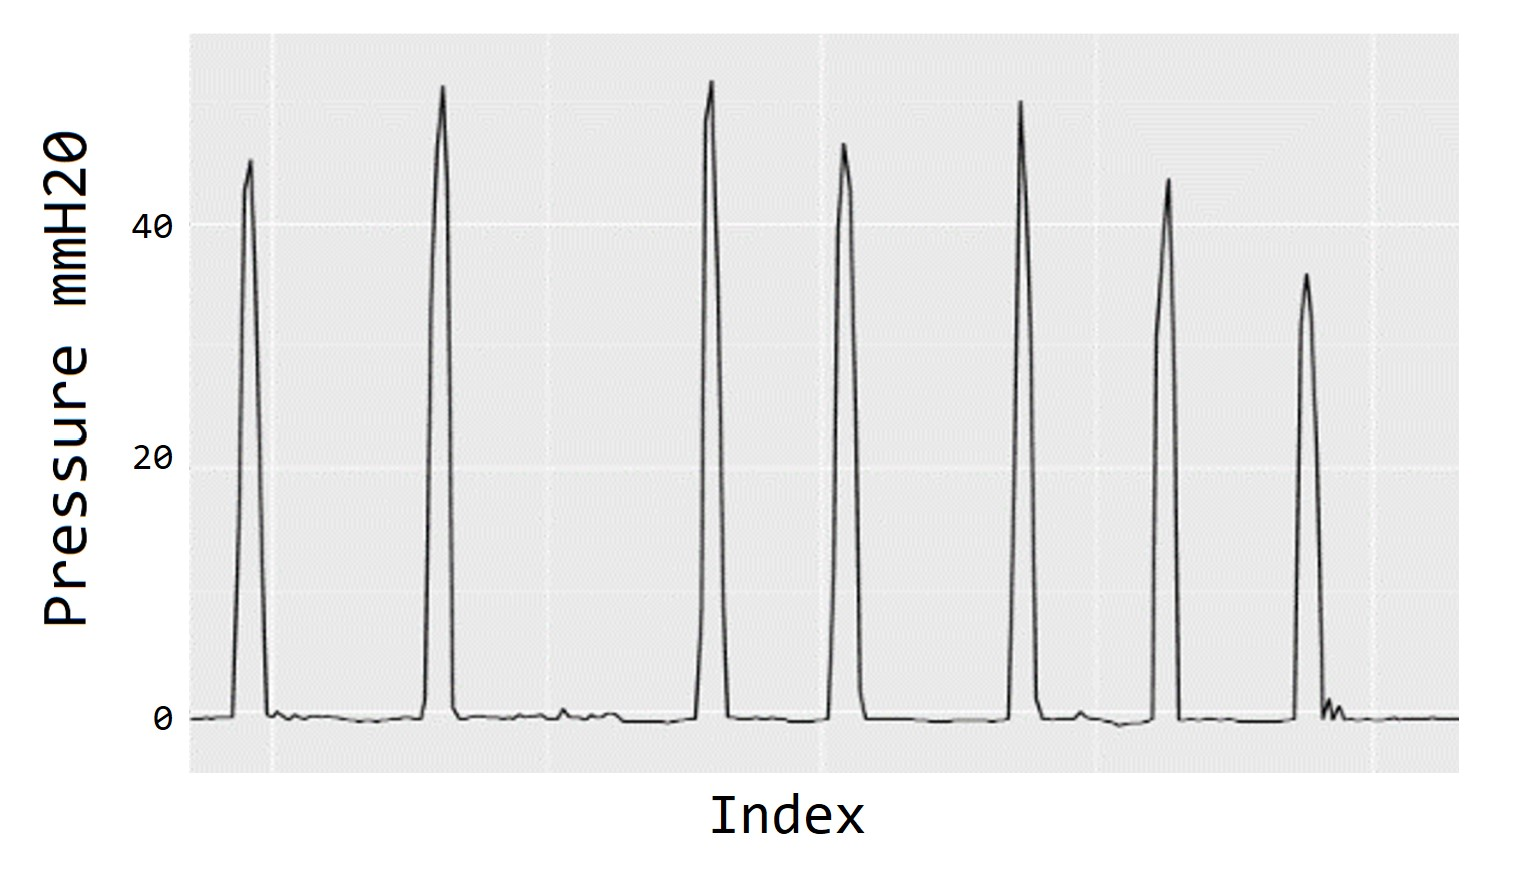
\includegraphics[width=0.9\textw%idth]{individual_breaths.jpg} % first %figure itself
%        \caption{A typical, %pre-processed ACT waveform. This %treatment is 20 seconds long and %contains 7 exhalation breaths.}
%        \label{fig:individual_breaths}
%    \end{minipage}\hfill
%    \begin{minipage}{0.48\textwidth}
%        \centering
%        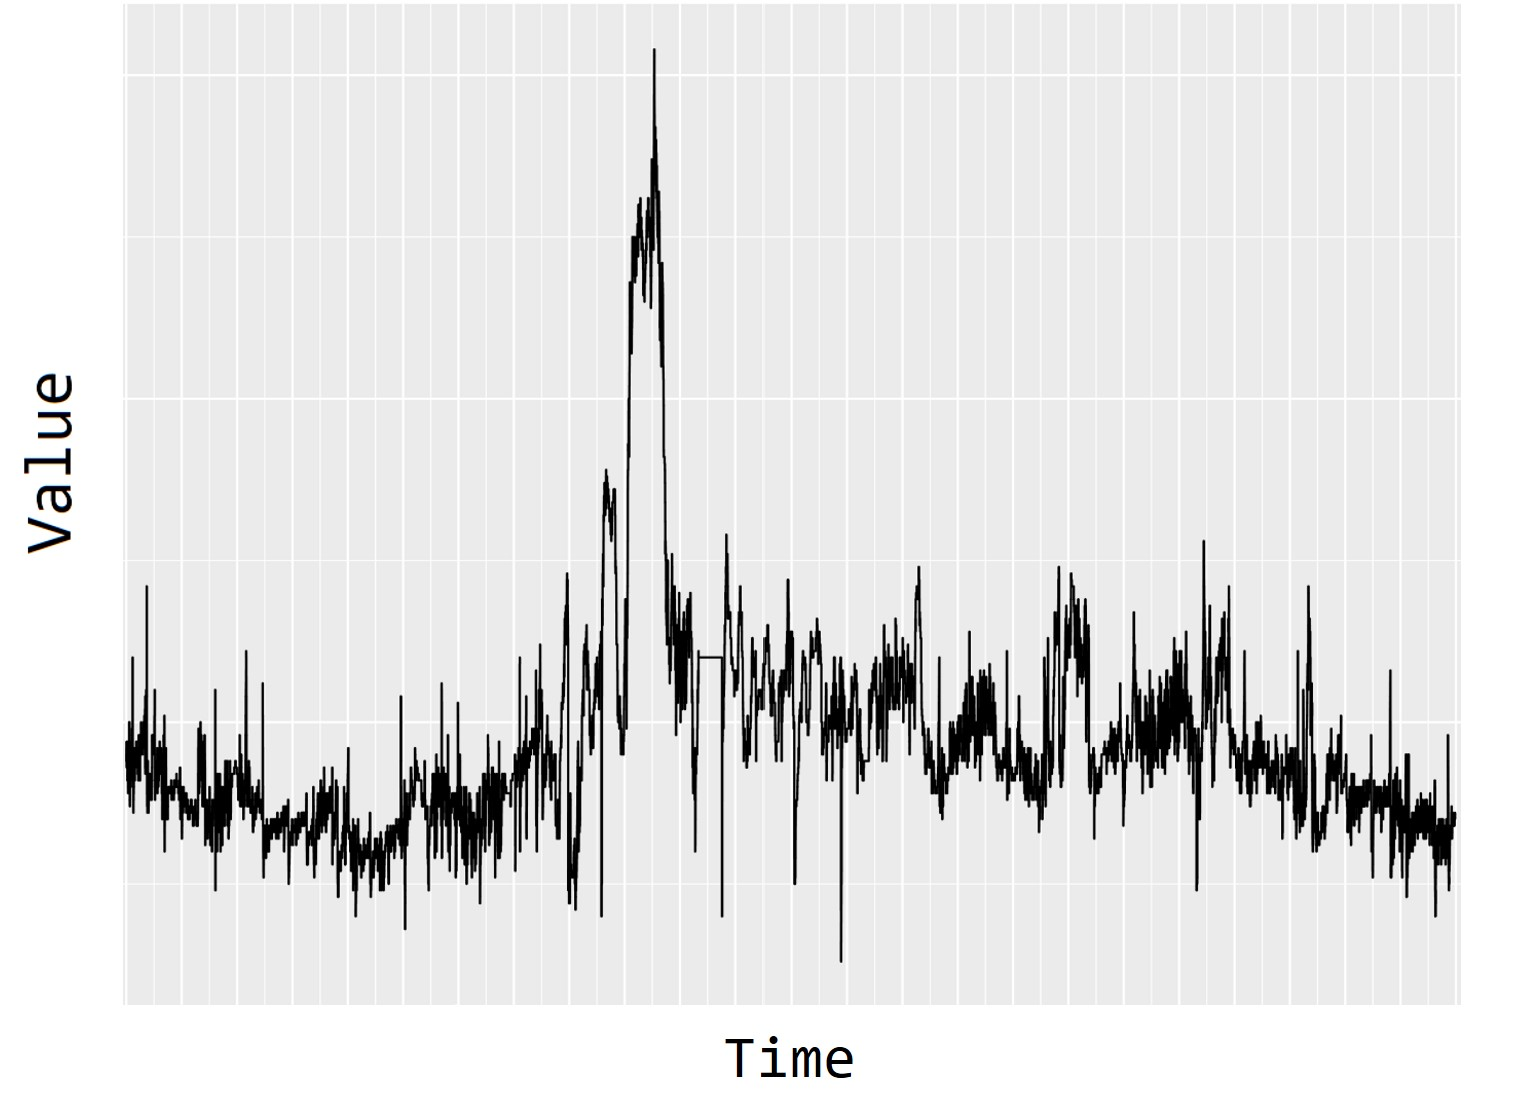
\includegraphics[width=0.88\text%width]{HR.jpg} % second figure itself
%        \caption{One day showing %heartrate data from the Fitbit with a %sustained period of heartrate in MVPA.}
%         \label{fig:HR}
%    \end{minipage}
%\end{figure}

We use breath amplitude standard deviation as a feature, in order to capture inconsistency or disorderliness in physiotherapy. Most features are on a per-treatment level. It is common for prescribed treatments to be skipped, and days with no treatments is an important signal itself. Several features were derived which captured missing data: treatment adherence to date, skipped days since last treatment, rolling adherence over 7 days. These features are on a per-day level, as participants are prescribed 1 or 2 treatments per day. We created a total of 27 features (Appendix \ref{appendix:actfeatures}) to describe ACT data. 

\subsubsection{Featurising Fitbit data}

The Fitbit activity tracker (Fitbit AltaHR) provided each participant’s step count per minute. While real-time heartbeat data would allow for a detailed analysis of heart rate waveforms, the Fitbit only provides average heart rate, with a variable sampling frequency ranging from 3 to 12 values per minute. To achieve consistent frequency and comparable values, the heart rate values were averaged for each minute. An example of heart rate data is shown in figure \ref{fig: Waveforms}.

We extracted high-level patterns from the minute-averaged waveforms at a day level. The heart rate and steps data sets were featurised using counts per day, such as number of minutes in moderate to vigorous intensity physical activities (MVPA) (heart rate above 120 bpm) per day. To account for missing data during times that the Fitbit was not worn, the wear percent of the Fitbit was calculated from the valid heart rate values. This measure was used to select only days with a substantial portion of data for the day (80~\% of wear time from 6~am to 6~pm), resulting in a dataset containing 9760 days used for analysis.  We created a total of 80 features (Appendix \ref{appendix:fitbitfeatures}) to describe Fitbit data. 

\subsection{Clustering physiotherapy data to find sub-types}  

We removed features which were highly correlated, and which were not verified by clinicians as being meaningful. We normalised all features and identified outliers using Tukey's method and removed less than 5~\%, with these cases being manually validated as device malfunctions or abnormal behaviour.  

We performed an initial assessment of clustering methods:  k-means, density-based spatial clustering of applications with noise (DBSCAN) and hierarchical clustering (HC) (see Appendices \ref{appendix:fitbitclusters} and \ref{appendix:actclusters}). For both ACT and Fitbit data, we found K-means clustering had the best performance in terms of silhouette width, Calinski-Harabasz index as well as having the most interpretable, clinically intuitive clusters. We selected k-means which we use for the rest of the analyses.

\subsubsection{Finding sub-types in ACT data}

Some features were excluded from clustering, but provided interesting physiotherapy insights: the number of sets in a treatment were expected to be influential in clustering, as a regular pattern of sets would show close adherence to physiotherapy advice. However we found that only 15\% of treatments had discernible sets, so this feature could not be used. The 7xx features used for clustering are shown in table X below, while the full list of features is shown in appendix \ref{appendix:actfeatures}. The Hopkins statistic for the data with the chosen features was 0.198, suggesting a high clustering tendency. 

The purpose of clustering into sub-types is to summarise how a participant is performing their ACT. We found the best clustering performance with k=4; the with centroid values are shown in table X below.


\begin{table}[H]
  \caption{ACT sub-types: clusters and centroid values. *: Fractional score calculated over a rolling 7 day period, all other features calculated at a treatment level.}
  \label{ACT_centroids}
  \centering
  \begin{tabularx}{17cm}{ X|X|X|X|X|X|X|X|X}
    \toprule
    \cmidrule(r){1-2}
    ACT sub-type & 
    Number of breaths & Mean breath duration (s) & SD breath duration (s) & Mean breath amplitude (mBar) &  SD breath amplitude (mBar) & Treatment duration (m) & 7-day treatment adherence* & 7-day breath adherence*  \\
    \midrule
    Alpha & 83.1645 & 1.1324091 & 0.9544094 & 19.13988 & 4.317706 & 11.31548 & 0.6117628 & 0.7350068\\
    Beta & 123.4091 & 0.8339444& 0.9706392 & 36.11484 & 9.864017 & 12.85468 & 0.7966647 & 1.2348730\\
    Gamma & 106.7632&     2.2134100 & 3.2749929 & 23.91718 & 6.191824 &  22.33150 &  0.7410448 &  1.1968865   \\
    Delta & 203.8484  &    1.1585528 & 1.2114907 &   21.55130 & 5.471787 & 26.88816 &  0.8643425 & 1.9809176 \\
    \bottomrule
    \end{tabularx}
\end{table}

The clusters identify sub-types in ACT data, for example the Alpha sub-type is characterised by near ideal (20 mBar) breath amplitude, low standard deviations (SD) indicating consistency in technique, and lower adherence, further interpretations in appendix \ref{appendix:actKmeansinterpretation}. These qualitative findings are consistent across two dimensionality reduction techniques, PCA and UMAP \cite{Mcinnes2018}. 

\subsubsection{ACT cluster validation }

Although the study is not complete, early results indicate that clusters are sensitive enough to track changes in some participants' adherence through different study interventions, as shown in figure ~\ref{fig:act_res}. We found that clustering was stable based on different data partitions, in terms of metrics such as silhouettes, and in terms of consistency of participant's cluster membership (see appendix \ref{appendix:actdatapartitions} and appendix \ref{appendix:actpatienttrajectories}).

\begin{figure}[!htb]
  \centering
  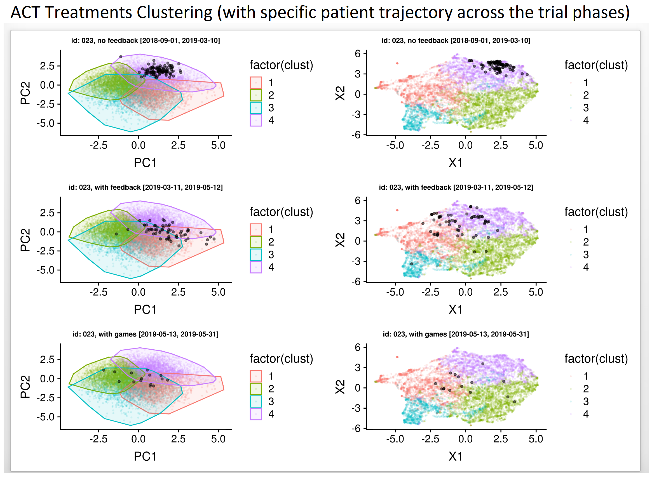
\includegraphics[]{fig_ACT_clust}
  \caption{the four ACT clusters overlaid with a single participant (black), showing that the participant’s cluster membership changes over time. Clustering results are visualised in 2-dimensions using PCA (left) and UMAP (right). The time points are before ACT feedback (number of registered breaths) is introduced (top), after ACT feedback is introduced (middle), and once computer gaming is introduced to ACT routine (bottom). Each point represents one treatment of one participant. }
  \label{fig:act_res}
\end{figure}

\subsubsection{Finding sub-types in Fitbit data} 

The purpose of clustering into sub-types is to summarise each participant's steps and heart rate waveforms, using a dataset containing 9760 days. 

\subsubsubsection{Heart rate clusters}

The following were used as features for heart rate clustering: the number of minutes with heart rate higher than 120, coefficient of variation for heart rate values per day, number of time heart rate exceeds 100 and 120, and the median average hourly heart rate. The Hopkins statistic for the data with the chosen features was: 0.062, suggesting a high clustering tendency. We found the best clustering performance with k=5, with clusters shown in figure \ref{fig:HRclusters}. The heart rate cluster centroid values are shown in Figure \ref{fig:hrBoundaries}. The clusters identify sub-types in heart rate data, for example the M1 sub-type is characterised Waveforms with high variability and periods with spikes above 120 bpm (see appendix \ref{appendix:hrclusters} for more details).  

\begin{figure}
    \centering
    \begin{minipage}{0.45\textwidth}
        \centering
        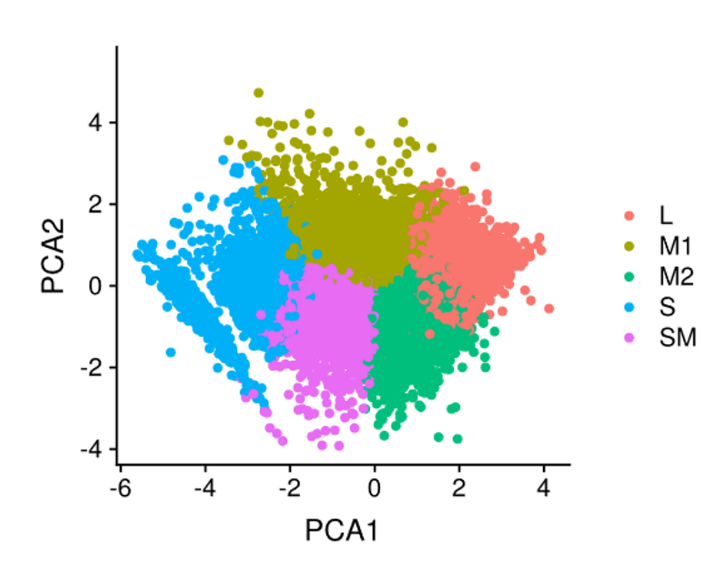
\includegraphics[width=0.9\textwidth]{HRclusters.png} % first figure itself
        \caption{PCA representation of the five heart rate clusters.}
        \label{fig:HRclusters}
    \end{minipage}\hfill
    \begin{minipage}{0.45\textwidth}
        \centering
        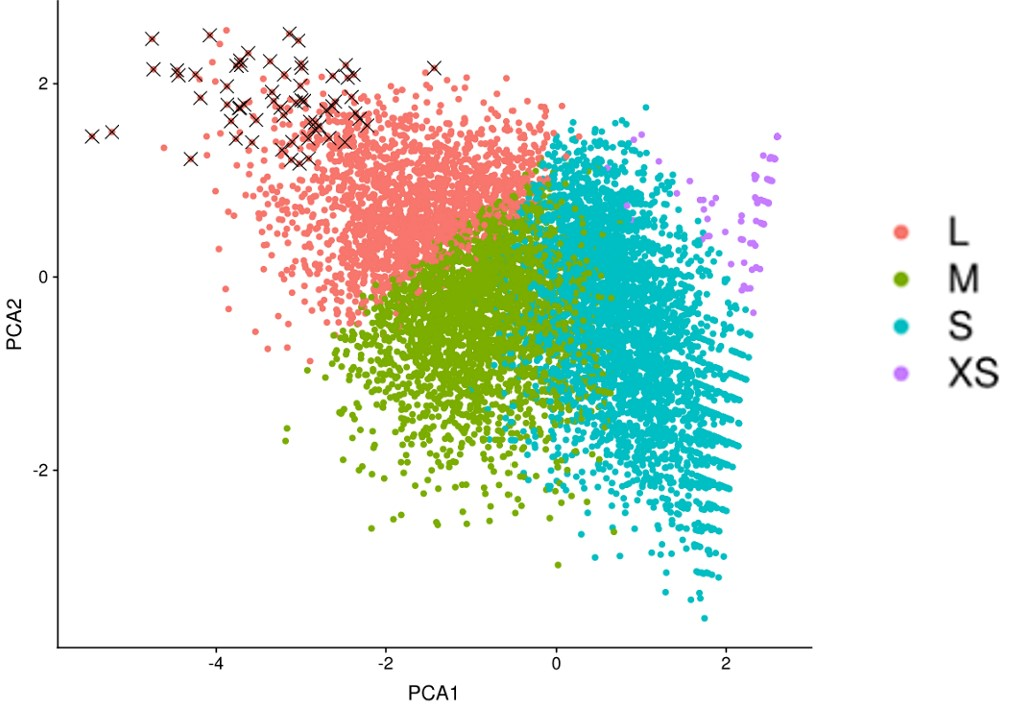
\includegraphics[width=0.9\textwidth]{FitbitClusterValidation.jpg} % second figure itself
        \caption{Steps clusters displayed on the first two principle components. Crosses are days with daily cadence above 30 which are all part of the L cluster.}
 \label{fig:FitbitClusterValidation}
    \end{minipage}
\end{figure}

\begin{figure}[H]
  \centering
  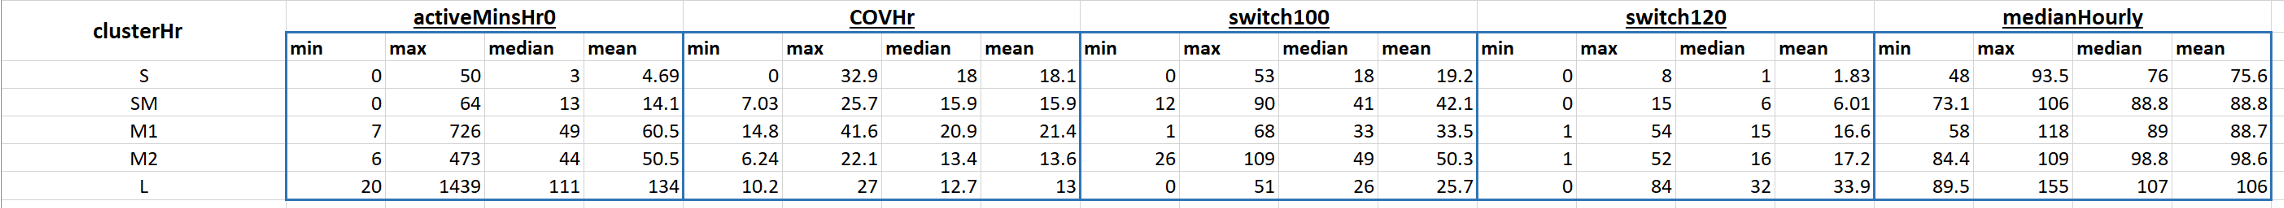
\includegraphics[scale=0.5]{hr_cluster_boundaries.png}
  \caption{Heart rate Cluster Boundaries}
  \label{fig:hrBoundaries}
\end{figure}

\subsubsubsection{Steps clusters}

The following features were used for clustering steps: number of minutes with step count higher than 100 for at least 5 consecutive minutes, mean step count per hour, step cadence for periods in MVPA, and number of hours in the day with 0~< ~step~count~<~500. The Hopkins statistic for the data with the chosen features was: 0.13375, suggesting a high clustering tendency. Four clusters were chosen, including one for missing data with the cluster boundaries shown in Figure \ref{fig:stepsBoundaries} (see appendix \ref{appendix:stepsclusters}).

\begin{figure}[H]
  \centering
  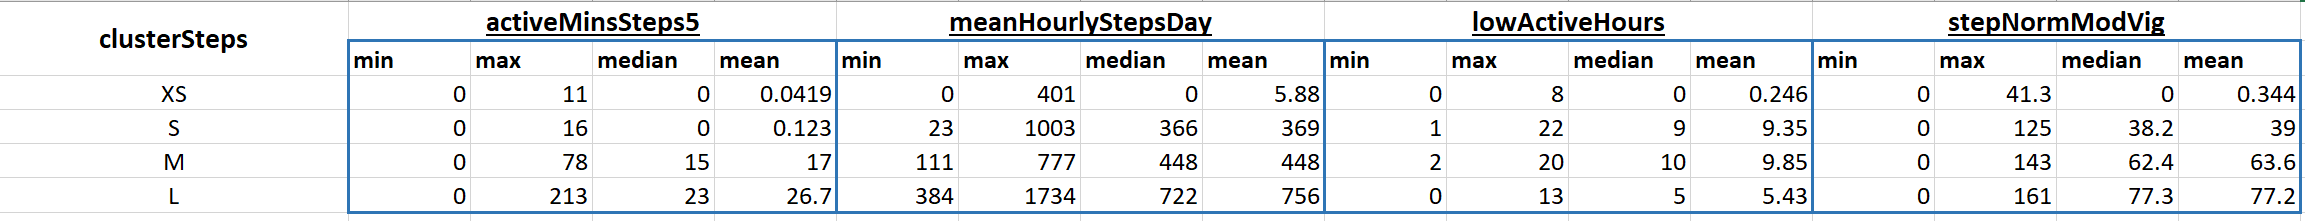
\includegraphics[scale=0.5]{steps_cluster_boundaries.png}
  \caption{Steps Cluster Boundaries}
  \label{fig:stepsBoundaries}
\end{figure}


\subsubsection{Fitbit cluster validation }

Steps and heart rate clusters were validated with clinical experts and found to be meaningful and useful ways to categorise the waveforms. Individual waveforms such as figure \ref{fig:HR} were manually inspected together with the cluster boundaries to ensure consistency across cluster interpretations and the actual cluster characteristics. Certain expected conditions were checked against the cluster labels and plotted using the PCA graph such as figure \ref{fig:FitbitClusterValidation}, which shows that all days with a cadence above 30, do indeed fall into the L cluster. 

\section{Discussion and conclusion} 

Project [Anonymised] involves collecting novel data about how CF physiotherapy advice on ACTs and physical activity is adhered to in everyday life, information which has never been available to physiotherapists.  In close collaboration with CF experts, we developed methods to interrogate and make sense of this data. Project [Anonymised] is an ongoing study, with participation lasting 18 months. 8 months into the trial we do not draw any conclusions, as we do not have an equal number of days of data from patients recruited over 8 months. Instead, we present a framework for analysis, which will empower clinicians to understand how physiotherapy advice is actually adhered to, and interpret the impact of interventions such as gamification when the trial is complete. Our framework involves processing the ACT and Fitbit data, deriving clinically meaningful features from it which characterise this novel data, and then using unsupervised clustering to find sub-types of this data. The clusters provide a useful way of tracking participants' trajectories across sub-types over time. In future the ACT and Fitbit features can be combined with each other, and with clinical data, to understand what type of physiotherapy leads to better clinical outcomes. The analysis of this data could help lead to more personalised treatment for CF, which could reduce treatment burden and improve health outcomes.


\bibliographystyle{abbrv}
% include your .bib file
\bibliography{fizzyo}

\newpage
\section*{Appendices}
\appendix

\section{Table of physical activity data features}
\label{appendix:fitbitfeatures}

\begin{longtable}{  n | d }
\toprule
\cmidrule(r){1-2}
\textbf{Fitbit features} & \textbf{Feature description} \\
\midrule
\endfirsthead
Minutes wear & Number of minutes in a day with heartrate value present \\
\midrule
Percentage of wear & $\frac{\textit{Minutes wear}}{24\cdot60}\cdot100\%$\\
\midrule
Wear during sleep & Indicator value: 1,  worn during sleep or 0, otherwise \\
\midrule
Active hours & Number of hours with a step count > 500  \\
\midrule
Low active hours & Number of hours with a step count < 500  \\
\midrule
Mean hourly steps & Average of hourly step count \\
\midrule
Step count & Total step count per day \\
\midrule
Normalised step count & Rate of steps per minute when fitbit is worn $\frac{\textit{Step Count}}{\textit{Minutes Worn}}$ \\
\midrule
 Step active minutes $k$, for $k\in \{0,2,5,10,20\}$ & Number of active minutes in a day. A minute is considered active if it has a step count > 100 and is part of a sequence of at least $k$ consecutive minutes with step count > 100. Note that for $k=0$ there is no restriction on the number of consecutive minutes\\
\midrule
Step active minutes during waking period & Number of minutes with step > 100 from 6am to midnight \\
\midrule
Step coefficient of variation & Coefficient of variation of minute step counts $CoV = \frac{\sigma (\textit{Step count})}{\mu (\textit{Step count})} \cdot 100$ \\
 \midrule
 Normalised step count for periods of : &  Rate of steps per minute when the heartrate is: \\
 - moderate activity & - between 120 and 140. \\ 
 - vigorous activity & - above 140. \\
 - moderate and vigorous activity & - above 120. \\
 - non-moderate and non-vigorous activity & - below 120.\\
 \midrule
 Resting heartrate proxy & Mean of the 5 minutes with the lowest heartrate average \\
 \midrule
Heartrate active minutes $k$, for $k\in \{0,2,5,10,20\}$ & Number of active minutes in a day. A minute is considered active if it has heartrate > 120 and is part of a sequence of at least $k$ consecutive minutes with heartrate > 120.\\
\midrule
Heartrate active minute during waking period & Number of minutes with heartrate > 120 from 6am to midnight \\
\midrule
Heartrate coefficient of variation & Coefficient of variation for heartrate minute averages $CoV = \frac{\sigma (\textit{Heartrate})}{\mu (\textit{Heartrate})} \cdot 100$ \\
 \midrule
 Number of switches above threshold $t$, for $t\in \{100,120,140\}$ & Number of times the heartrate goes above the threshold $t$ from below this threshold.\\ 
 \midrule
 Step and heartrate active minutes $k$, for $k\in \{0,2,5,10,20\}$ & Number of active minutes in a day. A minute is considered active if it has a step count > 100 and heartrate > 120 and is part of a sequence of at least $k$ consecutive minutes which satisfy both conditions. \\
\midrule
Hourly Max/Min/Median heart rate & Maximum, minimum and median of average hourly heartrate. \\
\bottomrule
\end{longtable}

\section{Table of ACT treatment features}
\label{appendix:actfeatures}

\begin{longtable}{ n|d}
\toprule
\cmidrule(r){1-2}
\textbf{ACT features} & \textbf{Feature description} \\
\midrule
Breath count & Number of breaths the person has made though an ACT device during a treatment. A breath is counted if its maximum amplitude is above the threshold of 8 mm H2O.\\
 \midrule
 Mean/Min/Max/Standard Deviation of breath amplitude & Statistics of breath amplitude (in mm H2O) during an ACT treatment. \\
  \midrule
 Mean/Min/Max/Standard Deviation of breath duration & Statistics of breath duration (in seconds) during an ACT treatment. \\
 \midrule
 Break count & Number of breaks (between breaths) in a treatment. \\
 \midrule
 Mean/Min/Max/Standard Deviation of breath duration & Statistics of duration (in seconds) of breaks between breaths in an ACT treatment. \\
 \midrule
 Set count & Number of sets in a treatment. Prescribed treatment may have up to 10 sets. Set is a group of breaths separated by huffing and coughing activity. \\
 \midrule
 Pressure readings count & Number of pressure reading registered by ACT device during a treatment. Used to filter out "test" device sessions that are not part of a treatment. \\
 \midrule
 Pressures readings completeness score & Data completeness score for the day If a treatment has less than 150 pressure readings it's completeness score is 0. \\
 \midrule
 Treatment duration & Treatment duration (in minutes). \\
 \midrule
 Treatment daily adherence score & Number of completed treatments out of the prescribed ones (for the given day). \\
 \midrule
 Breath count daily adherence score & Number of registered breaths across all treatments for the given day out of the prescribed amount of breaths. \\ 
 \midrule
 Treatment rolling weekly adherence score & Number of completed treatments during the last 7 days (for a given date) out of the prescribed number of treatments for this period. \\
 \midrule
 Breath count rolling weekly adherence score & Number of registered breaths across all treatments during the last 7 days (for a given date) out of the prescribed amount of breaths for this period. \\ 
 \midrule
 Treatment weekly adherence score & Number of completed treatments during the last calendar week (for a given date) out of the prescribed number of treatments for this period. \\
 \midrule
 Breath count weekly adherence score & Number of registered breaths across all treatments during the last calendar week(for a given date) out of the prescribed amount of breaths for this period.\\
 \midrule
 Cumulative adherence score & Cumulative adherence score to date. How many in total treatments patient done over a period (since the beginning of the study out the prescribed amount. \\
 \midrule
 Breathing time percentage & Percentage of time in a treatment spent on an exhalation \\
 \midrule
 Skipped days count & Skipped days since the last treatment. \\
 \bottomrule
\end{longtable}

\section{Cluster results and metrics for physical activity data}
\label{appendix:fitbitclusters}
\subsection{Steps clusters}
\label{appendix:stepsclusters}
\subsubsection{K-means Clustering}
\label{appendix:stepsKmeans}

\paragraph{Clusters Interpretation}
Clusters interpretation for the four steps clusters can be seen in Table \ref{steps_inter}.

\begin{table}[H]
  \caption{Steps Clusters Interpretation}
  \label{steps_inter}
  \centering
  \begin{tabular}{ c|d }
    \toprule
    \cmidrule(r){1-2}
    \textbf{Cluster name} & \textbf{Cluster Interpretation} \\
    \midrule
    XS & Waveforms with very little steps activity or high amount of missing data \\
    \midrule
    S & Moderate step activity, consistent cadence with few periods of high activity\\
    \midrule
    M & Consistent moderate to high step rate with a period of sustained high step activity \\
    \midrule
    L & High step rate with longer periods of sustained high step activity \\
    \bottomrule
    \end{tabular}
\end{table}

\paragraph{Clusters Boundaries}
Clusters boundaries  for the four steps clusters can be seen in Table \ref{steps_boundaries}.

\begin{table}[H]
  \caption{Steps clusters boundaries - mean, median, min, max}
  \label{steps_boundaries}
  \centering
  \begin{tabular}{p{4cm}*{5}{|p{1cm}}}
    \toprule
    \multicolumn{2}{c|}{\backslashbox{Boundaries}{Cluster Name}} & \textbf{XS} & \textbf{S} & \textbf{M} & \textbf{L} \\
    \midrule
    \multirow{4}{4cm}{\textbf{Step Active Minutes 5}} & mean & 0.0419 & 0.123 & 17 & 26.7 \\ 
    & median & 0 & 0 & 15 & 23\\ 
    & min & 0 & 0 & 0 & 0 \\ 
    & max & 11 & 16 & 78 & 213 \\ 
    \hline
    \multirow{4}{4cm}{\textbf{Mean Hourly Step}} & mean & 5.88 & 369 & 448 & 756 \\
    & median & 0 & 366 & 448 & 722 \\
    & min & 0 & 23 & 111 & 384 \\
    & max & 401 & 1003 & 777 & 1734 \\
    \hline
    \multirow{4}{4cm}{\textbf{Low Active Hours}} & mean & 0.246 & 9.35 & 9.85 & 5.43 \\
    & median & 0 & 9 & 10 & 5\\
    & min & 0 & 1 & 2 & 0 \\
    & max & 8 & 22 & 20 & 13\\
    \hline
    \multirow{4}{4cm}{\textbf{Step cadence for periods of moderate and vigorous activity}} & mean & 0.344 & 39 & 63.6 & 77.2 \\
    & median & 0 & 38.2 & 62.4 & 77.3 \\
    & min & 41.3 & 125 & 143 & 161 \\
    & max & 0 & 0 & 0 & 0 \\
    \bottomrule
    \end{tabular}
\end{table}

\paragraph{Cluster Metrics}
Calinski-harabasz index for the steps clusters is 6021.14 .

\begin{table}[H]
  \caption{Steps clusters Metrics Kmeans}
  \label{steps_metrics}
  \centering
  \begin{tabular}{ c|c|c}
    \toprule
    \cmidrule(r){1-2}
    Cluster name & Cluster Size & Average Silhouette width \\
    \midrule
    XS & 1099 & 0.95 \\
    S & 3942 & 0.34 \\
    M & 2737 & 0.27 \\
    L & 1982 & 0.24 \\
    \bottomrule
    \end{tabular}
\end{table}

\subsubsection{Hierarchical Clustering with complete linkage}
\label{appendix:stepsHC}
The clustering results using Hierarchical clustering with complete linkage on steps data displayed using the first two principal components can be seen in Figure \ref{fig:stepsClustersHC}. These clusters were not named and interpreted as the clusters results from Kmeans as the metrics did not shown promising results, hence their default numbering is shown.

\begin{figure}[H]
  \centering
  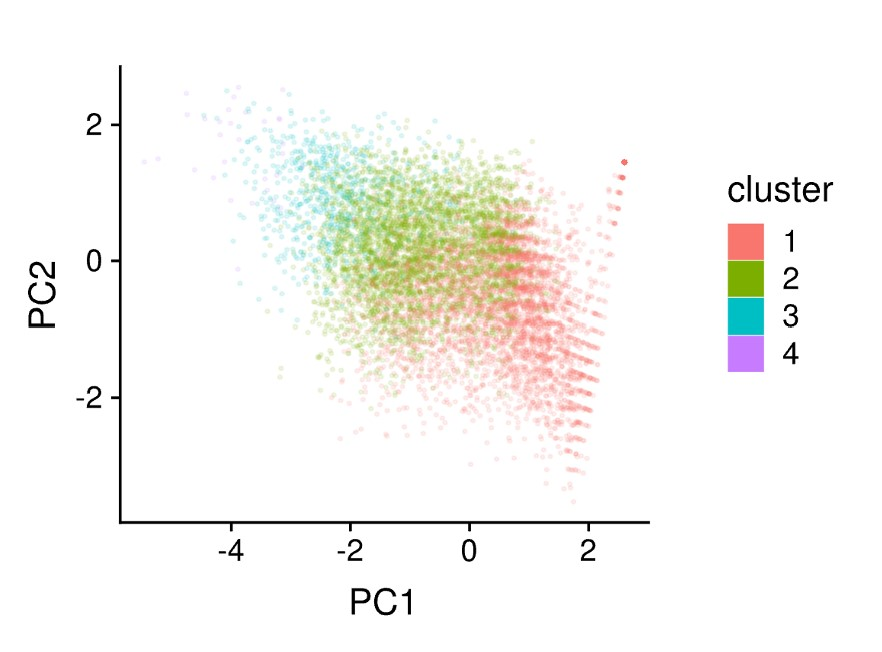
\includegraphics[]{steps_HC_results.jpg}
  \caption{Steps clusters displayed on the first two principle components obtained using Hierarchical clustering}
  \label{fig:stepsClustersHC}
\end{figure}

Calinski-harabasz index for the steps clusters is 1518.1865 .

\begin{table}[H]
  \caption{Steps clusters Metrics HC}
  \label{steps_metrics}
  \centering
  \begin{tabular}{ c|c|c}
    \toprule
    \cmidrule(r){1-2}
    Cluster number & Cluster Size & Average Silhouette width \\
    \midrule
    1 & 4996 & 0.12 \\
    2 & 4056 & 0.11 \\
    3 & 677 & 0.18 \\
    4 & 31 & 0.41 \\
    \bottomrule
    \end{tabular}
\end{table}

\subsection{Heartrate clusters}
\label{appendix:hrclusters}
\subsubsection{K-Means Clustering}
\label{appendix:hrKmeans}
\paragraph{Clusters Interpretation}
Clusters interpretations for the five heartrate clusters can be seen in Table \ref{hr_inter}.

\begin{table}[H]
  \caption{Heart rate Clusters Interpretation}
  \label{hr_inter}
  \centering
  \begin{tabular}{ c|d }
    \toprule
    \cmidrule(r){1-2}
    \textbf{Cluster name} & \textbf{Cluster Interpretation} \\
    \midrule
    S & Small heart rate values and heart rate consistently below 120 \\
    \midrule
    SM & Consistent variations around 100 with very few spikes in heart rate values \\
    \midrule
    M1 &  Waveform with high variability and periods with spikes above 120 \\
    \midrule
    M2 & Consistent variations around 100 with spikes in values above 120 \\
    \midrule
    L &  Large values around and above 120 \\
    \bottomrule
    \end{tabular}
\end{table}

\paragraph{Clusters Boundaries}
Clusters boundaries  for the heartrate clusters can be seen in Table \ref{hr_boundaries}.

\begin{table}[H]
  \caption{Heartrate clusters boundaries - mean, median, min, max}
  \label{hr_boundaries}
  \centering
  \begin{tabular}{p{4cm}*{6}{|p{1cm}}}
    \toprule
    \multicolumn{2}{c|}{\backslashbox{Boundaries}{Cluster Name}} & \textbf{S} & \textbf{SM} & \textbf{M1} & \textbf{M2} & \textbf{L} \\
    \midrule
    \multirow{4}{4cm}{\textbf{Heartrate Active Minutes 0}} & mean & 4.69 & 14.1 & 60.5 & 50.5 & 134 \\
    & median & 3 & 13 & 49 & 44 & 111 \\
    & min & 0 & 0 & 7 &  6 & 20\\
    & max & 50 & 64 & 726 & 473 & 1439 \\
    \hline
    \multirow{4}{4cm}{\textbf{Heartrate Coefficient of Variation}} & mean & 18.1 & 15.9 & 21.4 & 13.6 & 13 \\
    & median & 18 & 15.9 & 20.9 & 13.4 & 12.7 \\
    & min & 0 & 7.03 & 14.8 & 6.24 & 10.2 \\
    & max & 32.9 & 25.7 & 41.6 & 22.1 & 27 \\
    \hline
    \multirow{4}{4cm}{\textbf{Number of switches above 100}} & mean & 19.2 & 42.1 & 33.5 & 50.3 & 25.7\\
    & median & 18 & 41 & 33 & 49 & 26 \\
    & min & 0 & 12 & 1 & 26 & 0\\
    & max & 53 & 90 & 68 & 109 & 51 \\
    \hline
    \multirow{4}{4cm}{\textbf{Number of switches above 120}} & mean & 1.83 & 6.01 & 16.6 & 17.2 & 33.9 \\
    & median & 1 & 6 & 15 & 16 & 32 \\
    & min & 0 & 0 & 1 & 1 & 0\\
    & max & 8 & 15 & 54 & 52 & 84 \\
    \hline
    \multirow{4}{4cm}{\textbf{Median Hourly heartrate}} & mean & 75.6 & 88.8 & 88.7 & 98.6 & 106 \\
    & median & 76 & 88.8 & 89 & 98.8 & 107\\
    & min & 48 & 73.1 & 58 & 84.4 & 89.5\\
    & max & 93.5 & 106 & 118 & 109 & 155 \\
    \bottomrule
    \end{tabular}
\end{table}

\paragraph{Cluster Metrics}
Calinski-harabasz index for the heartrate clusters is 5090.37 .

\begin{table}[H]
  \caption{Heartrate clusters Metrics Kmeans}
  \label{hr_metrics}
  \centering
  \begin{tabular}{ c|c|c}
    \toprule
    \cmidrule(r){1-2}
    Cluster name & Cluster Size & Average Silhouette width \\
    \midrule
    S & 1246 & 0.28 \\
    SM & 1640 & 0.2 \\
    M1 & 2308 & 0.21 \\
    M2 & 2584 & 0.26 \\
    L & 1982 & 0.33 \\
    \bottomrule
    \end{tabular}
\end{table}

\subsubsection{Hierarchical Clustering with complete linkage}
\label{appendix:hrHC}

The clustering results using Hierarchical clustering with complete linkage for the heart rate data displayed using the first two principal component can be seen in Figure \ref{fig:hrClustersHC}. These clusters were not named and interpreted as the clusters results from Kmeans as the metrics did not shown promising results, hence their default numbering is shown.

\begin{figure}[H]
  \centering
  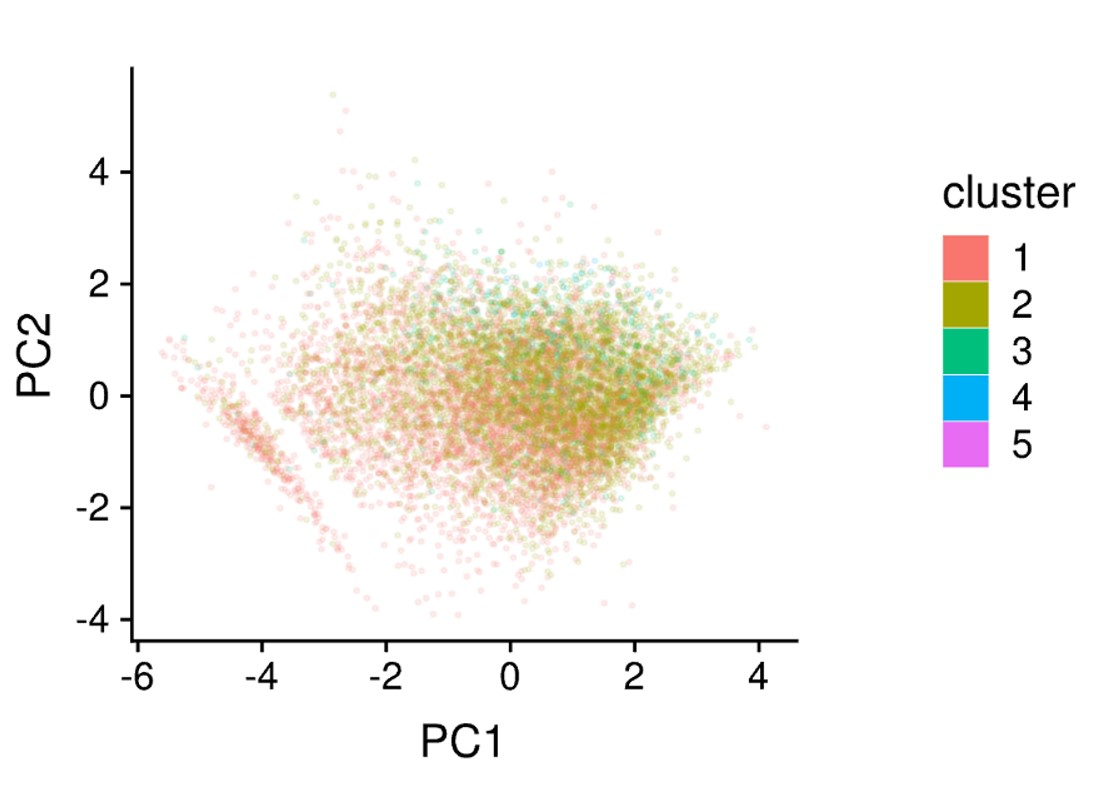
\includegraphics[]{hr_HC_results.jpg}
  \caption{Heart rate clusters displayed on the first two principle components obtained using Hierarchical clustering}
  \label{fig:hrClustersHC}
\end{figure}

Calinski-Harabasz index for the heart rate clusters is 135.51 .

\begin{table}[H]
  \caption{Heart rate clusters Metrics HC}
  \label{hr_metrics}
  \centering
  \begin{tabular}{ c|c|c}
    \toprule
    \cmidrule(r){1-2}
    Cluster number & Cluster Size & Average Silhouette width \\
    \midrule
    1 & 4221 & -0.07 \\
    2 & 4901 & -0.06 \\
    3 & 607 & -0.10 \\
    4 & 24 & 0.07 \\
    5 & 7 & -0.06 \\
    \bottomrule
    \end{tabular}
\end{table}

\newpage
\section{Cluster results and metrics for ACT treatments}
\label{appendix:actclusters}

The tables below show the metrics for the ACT treatment clusters.
\subsection{K-Means Clustering}
\label{appendix:actKmeans}
\subsubsection{K-Means Metrics and Number of Clusters}
\label{appendix:actKmeansmetrics}
The table below shows comparison of Average Silhouette width and Calinski-Harabasz index different number of clusters

\begin{table}[H]
  \caption{Clusters Metrics Kmeans vs Number of Clusters}
  \label{steps_metrics}
  \centering
  \begin{tabular}{ c|c|c}
    \toprule
    \cmidrule(r){1-2}
    Number of Clusters & Calinski-Harabasz index & Average Silhouette width \\
    \midrule
    3 & 2292 & 0.17 \\
    4 & 2208 & 0.18 \\
    5 & 1996 & 0.15 \\
    6 & 1830 & 0.15 \\
    \bottomrule
    \end{tabular}
\end{table}

\subsubsection{Cluster interpretation}
\label{appendix:actKmeansinterpretation}
Clustering with number clusters k=4 has combination of good performance (Average Silhouette width and Calinski-Harabasz index) and positive feedback from clinical team on cluster level granularity and clusters interpretability. 

If k is too low, the sub-types are not granular enough, if k is too high it becomes challenging to remember the characteristics of each sub-type.

 Based on these centroids, the four ACT sub-types, which we named alpha, beta, gamma and delta have the following interpretations: 

\begin{itemize}
\item Alpha (Cluster 1) - Treatments with exceptionally big breath counts and biggest treatment adherence.
\item Beta (Cluster 2) - Breath counts weekly adherence is on a lower side, treatments are short.
\item Gamma (cluster 3) -  Good breath counts and related breath weekly adherence, the breaths themselves have big standard deviation of duration.
\item Delta (Cluster 4) - Very good breath counts and related breath weekly adherence,  breaths are mostly short and powerful (with biggest standard deviation for amplitude), shorter treatments.
\end{itemize}

The clusters capture variability of ACT treatments patient do at home, for example we identified clusters that are characterized by big adherence or breath with higher amplitude.

\begin{figure}[H]
  \centering
  \caption{ACT clusters displayed on PCA and UMAP projections obtained using Kmeans clustering}
  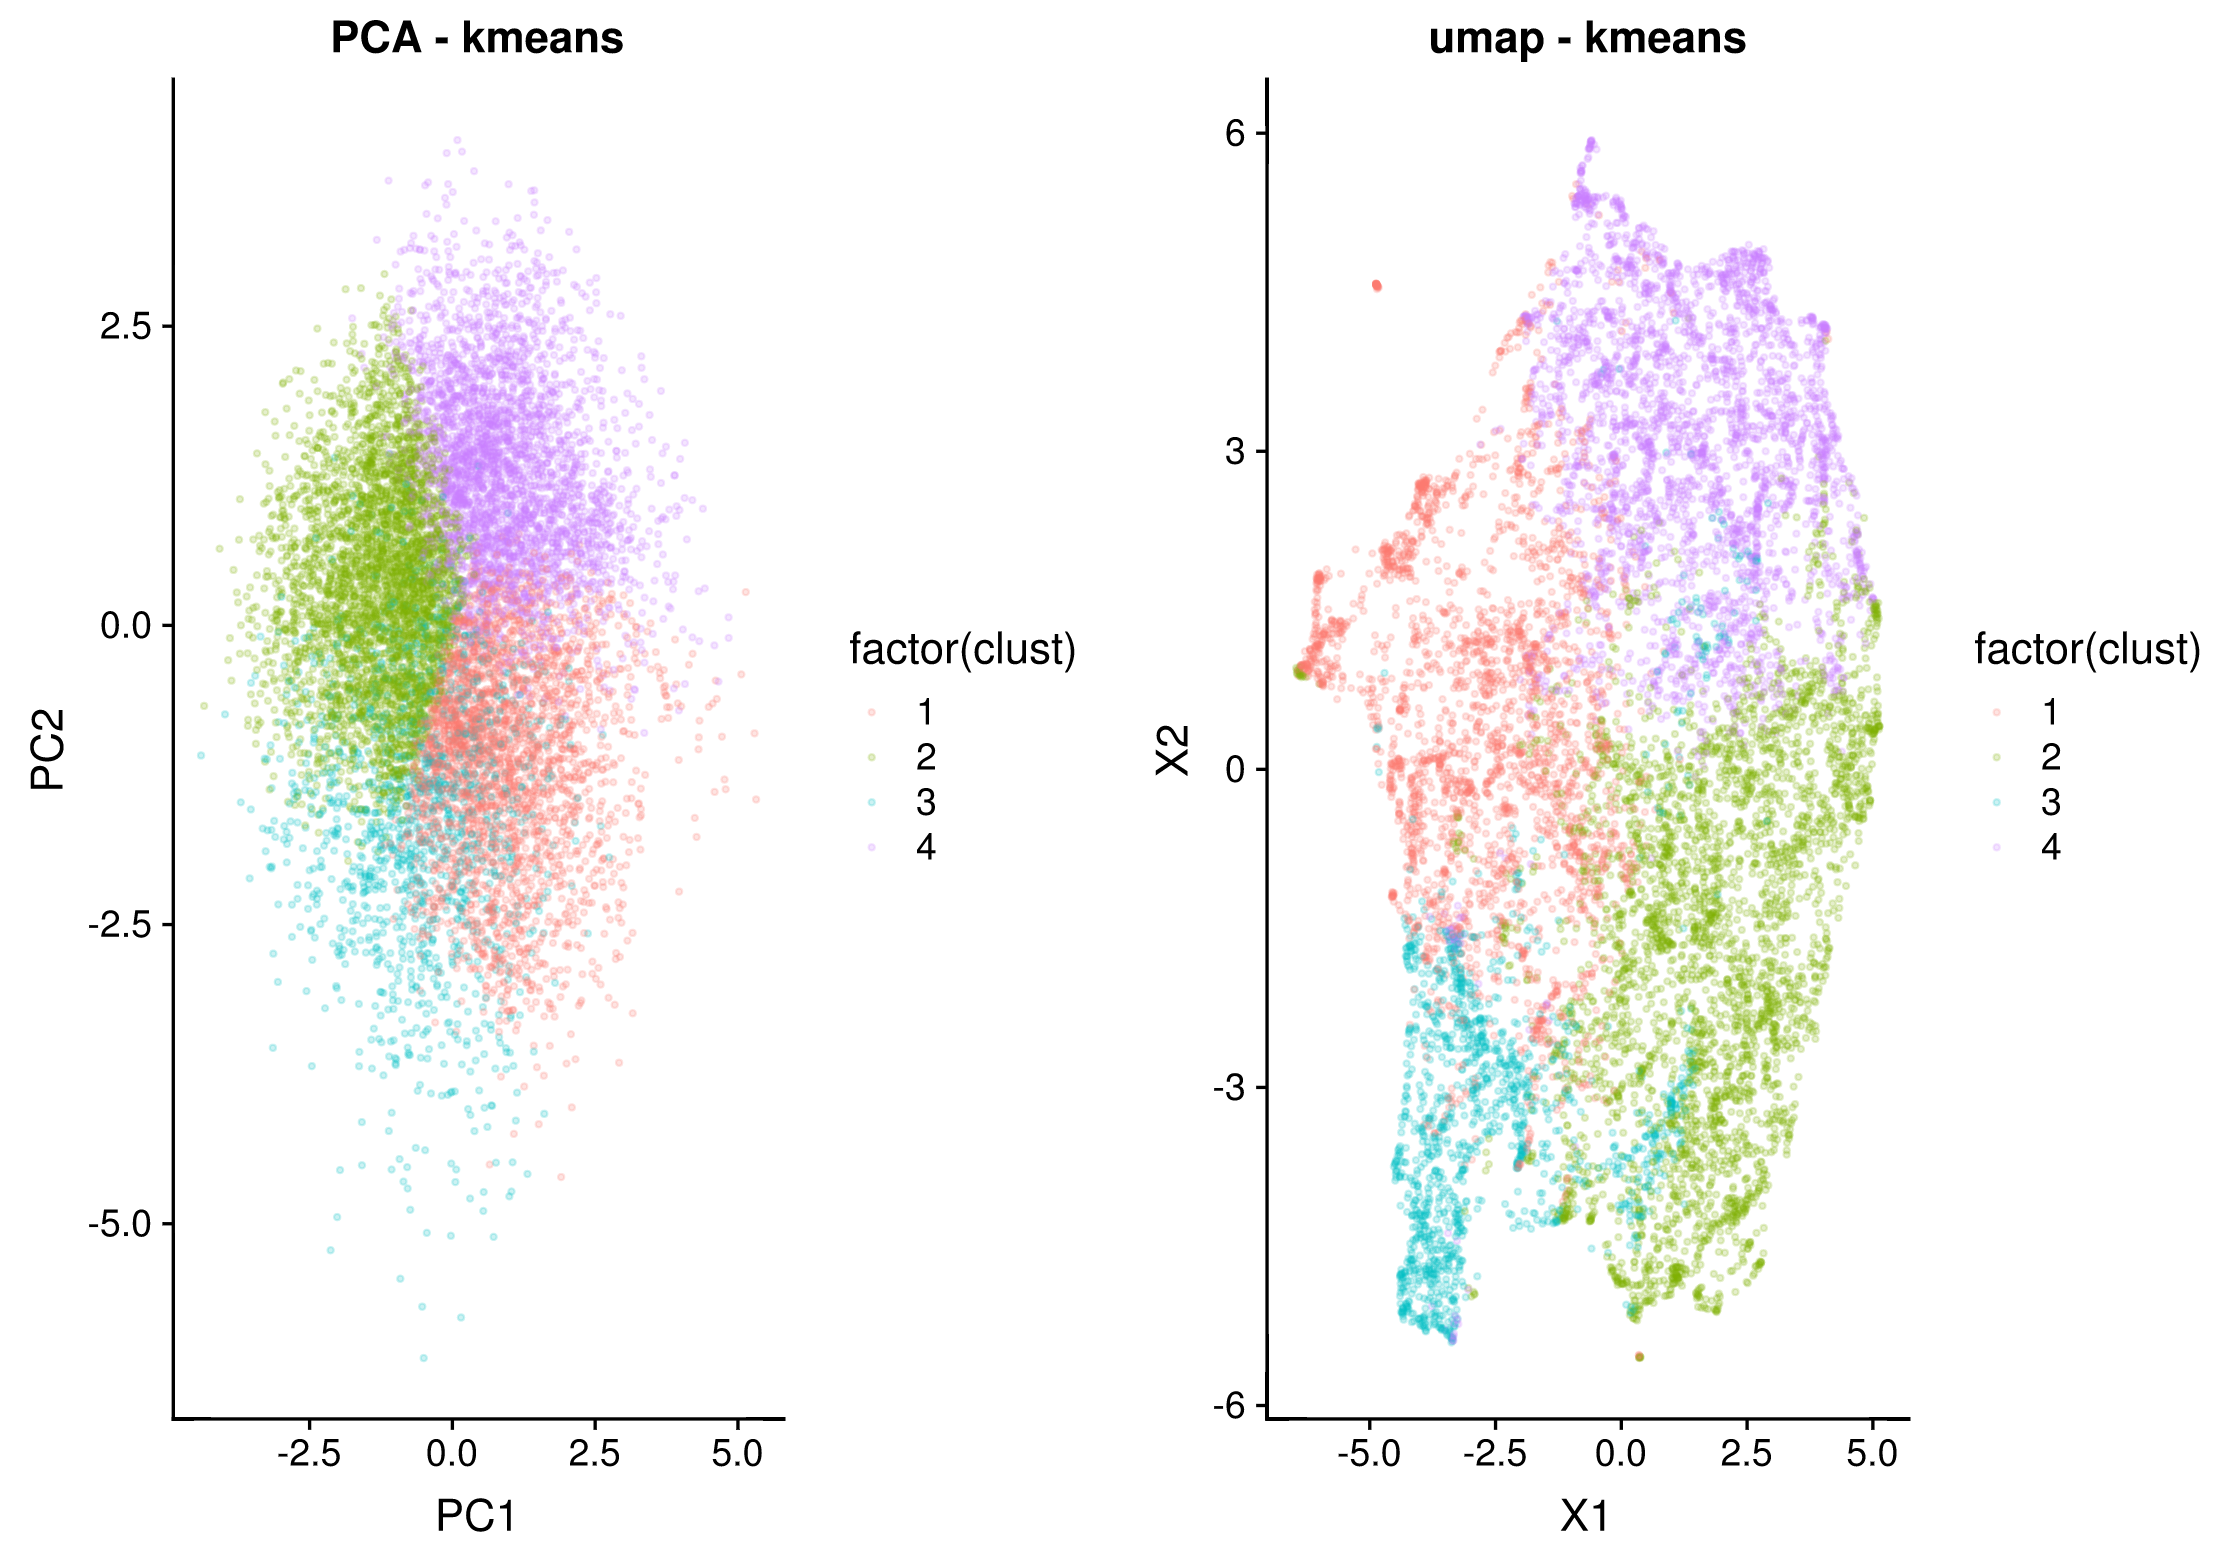
\includegraphics[scale=0.5]{fig_ACT_4_clusters.png}
  \label{fig:figACT4clusters}
\end{figure}


\subsection{Hierarchical Clustering}
\label{appendix:actHC}
Figure \ref{fig:figACTdent} shows the Dendrogram of ACT data demonstrating major splits for number of clusterts k = 2,3,5 and 6

\begin{figure}[H]
  \centering
  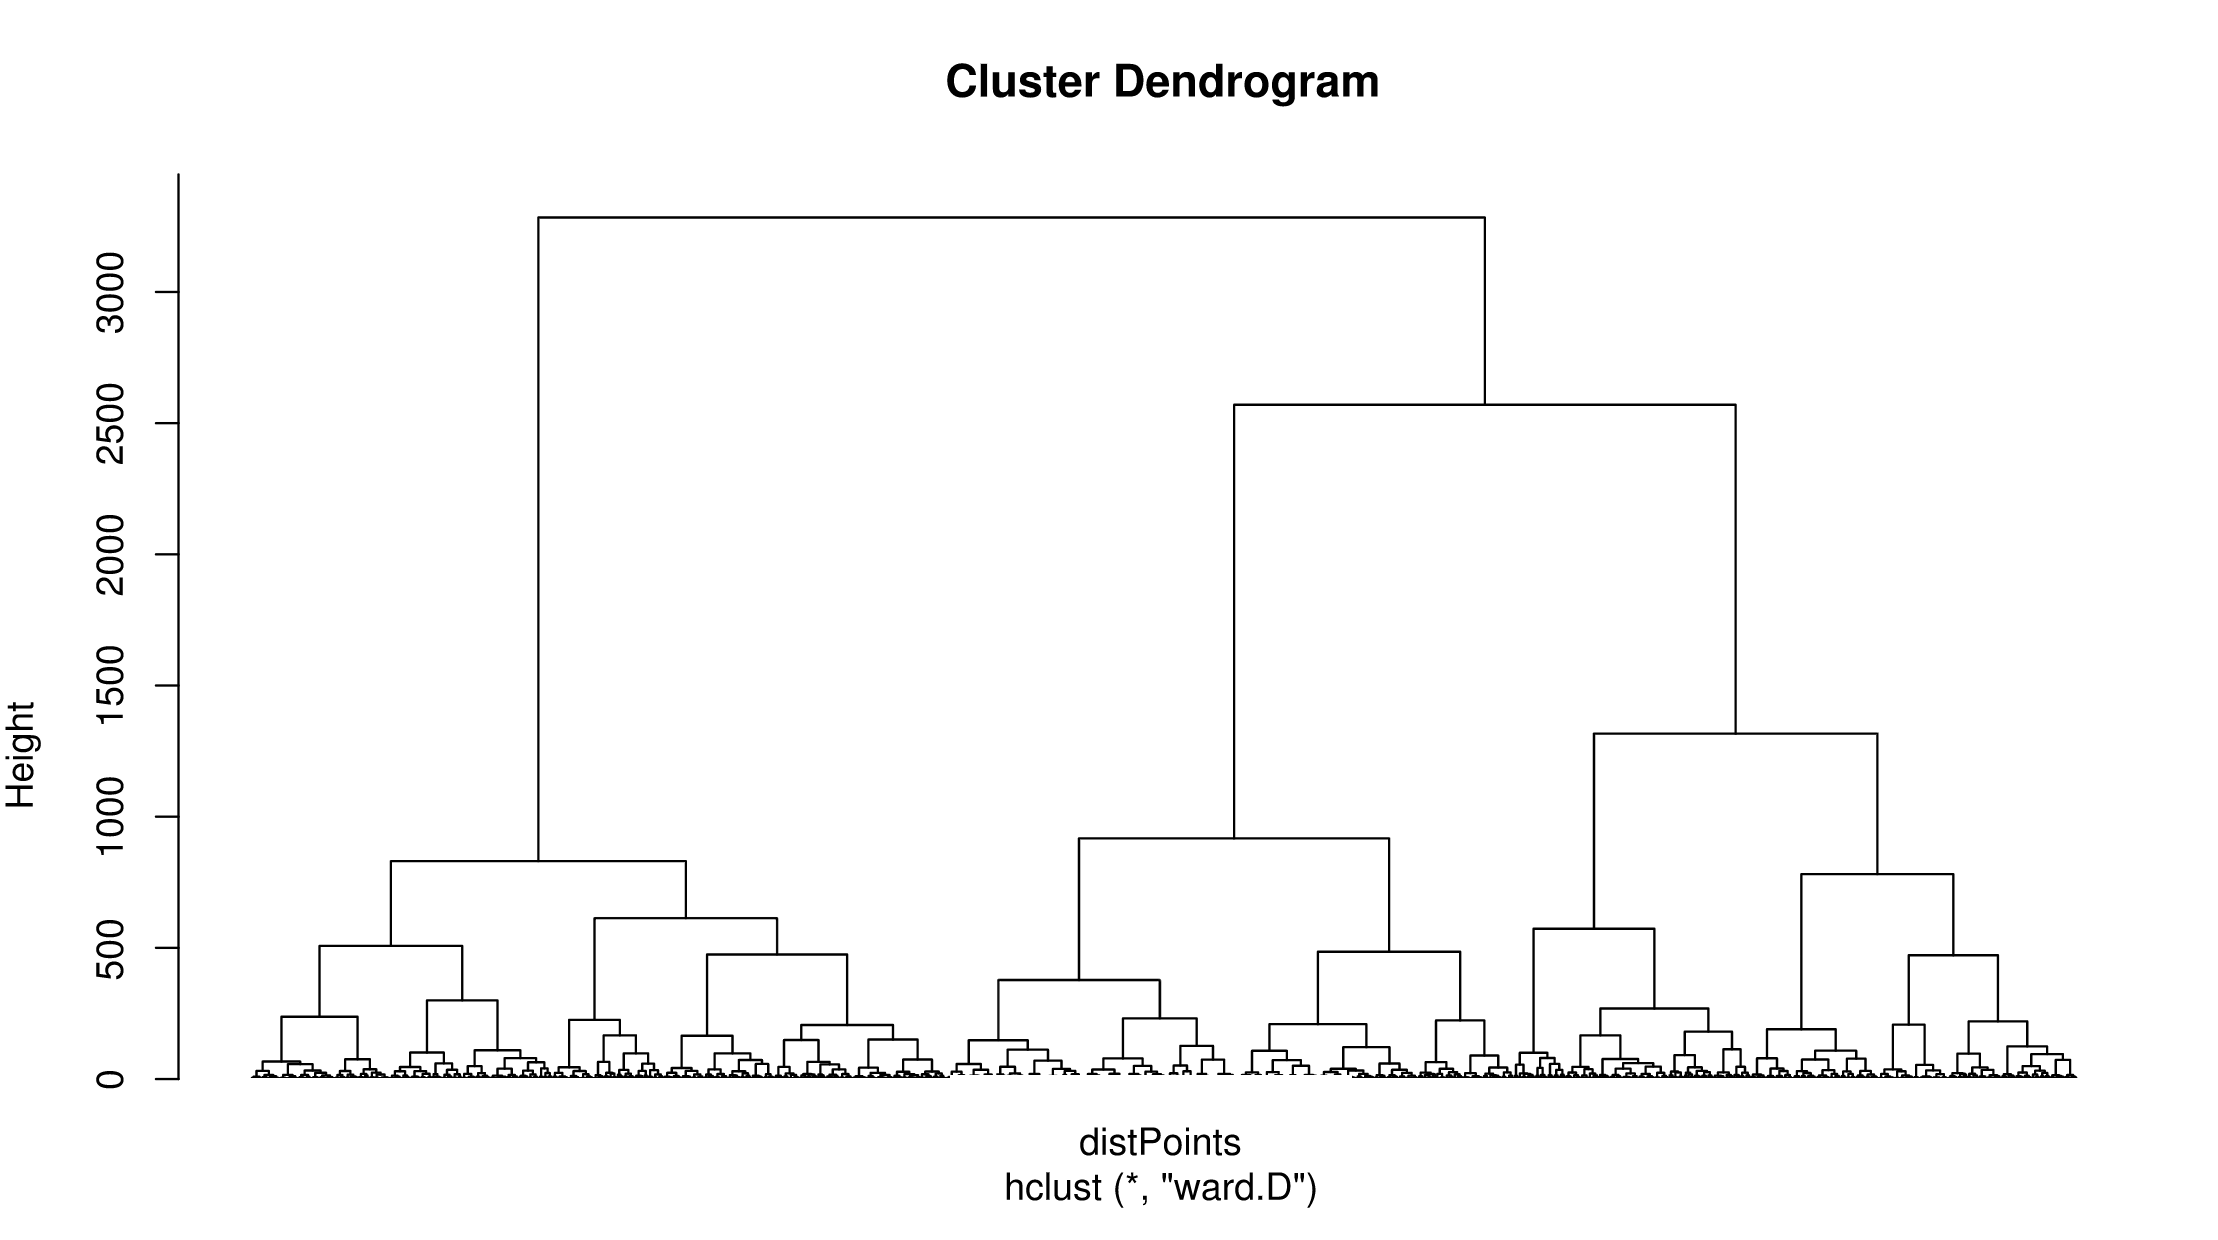
\includegraphics[scale=0.5]{fig_ACT_HC_dentogram.png}
  \caption{ Hierarchical Clustering Dendrogram for ACT data}
  \label{fig:figACTdent}
\end{figure}

The table \ref{tab:act_hc_clusters} shows comparison of Average Silhouette width and Calinski-Harabasz index different number of clusters.

\begin{table}[H]
  \caption{Clusters Metrics for Hierahical Clustering vs Number of Clusters}
  \label{tab:act_hc_clusters}
  \centering
  \begin{tabular}{ c|c|c}
    \toprule
    \cmidrule(r){1-2}
    Number of Clusters & Calinski-Harabasz index & Average Silhouette width \\
    \midrule
    3 & 1793 &  0.13\\
    4 & 1643 &  0.13\\
    5 & 1414 &  0.08\\
    6 & 1289 &  0.06 \\
    \bottomrule
    \end{tabular}
\end{table}

\begin{figure}[H]
  \centering
  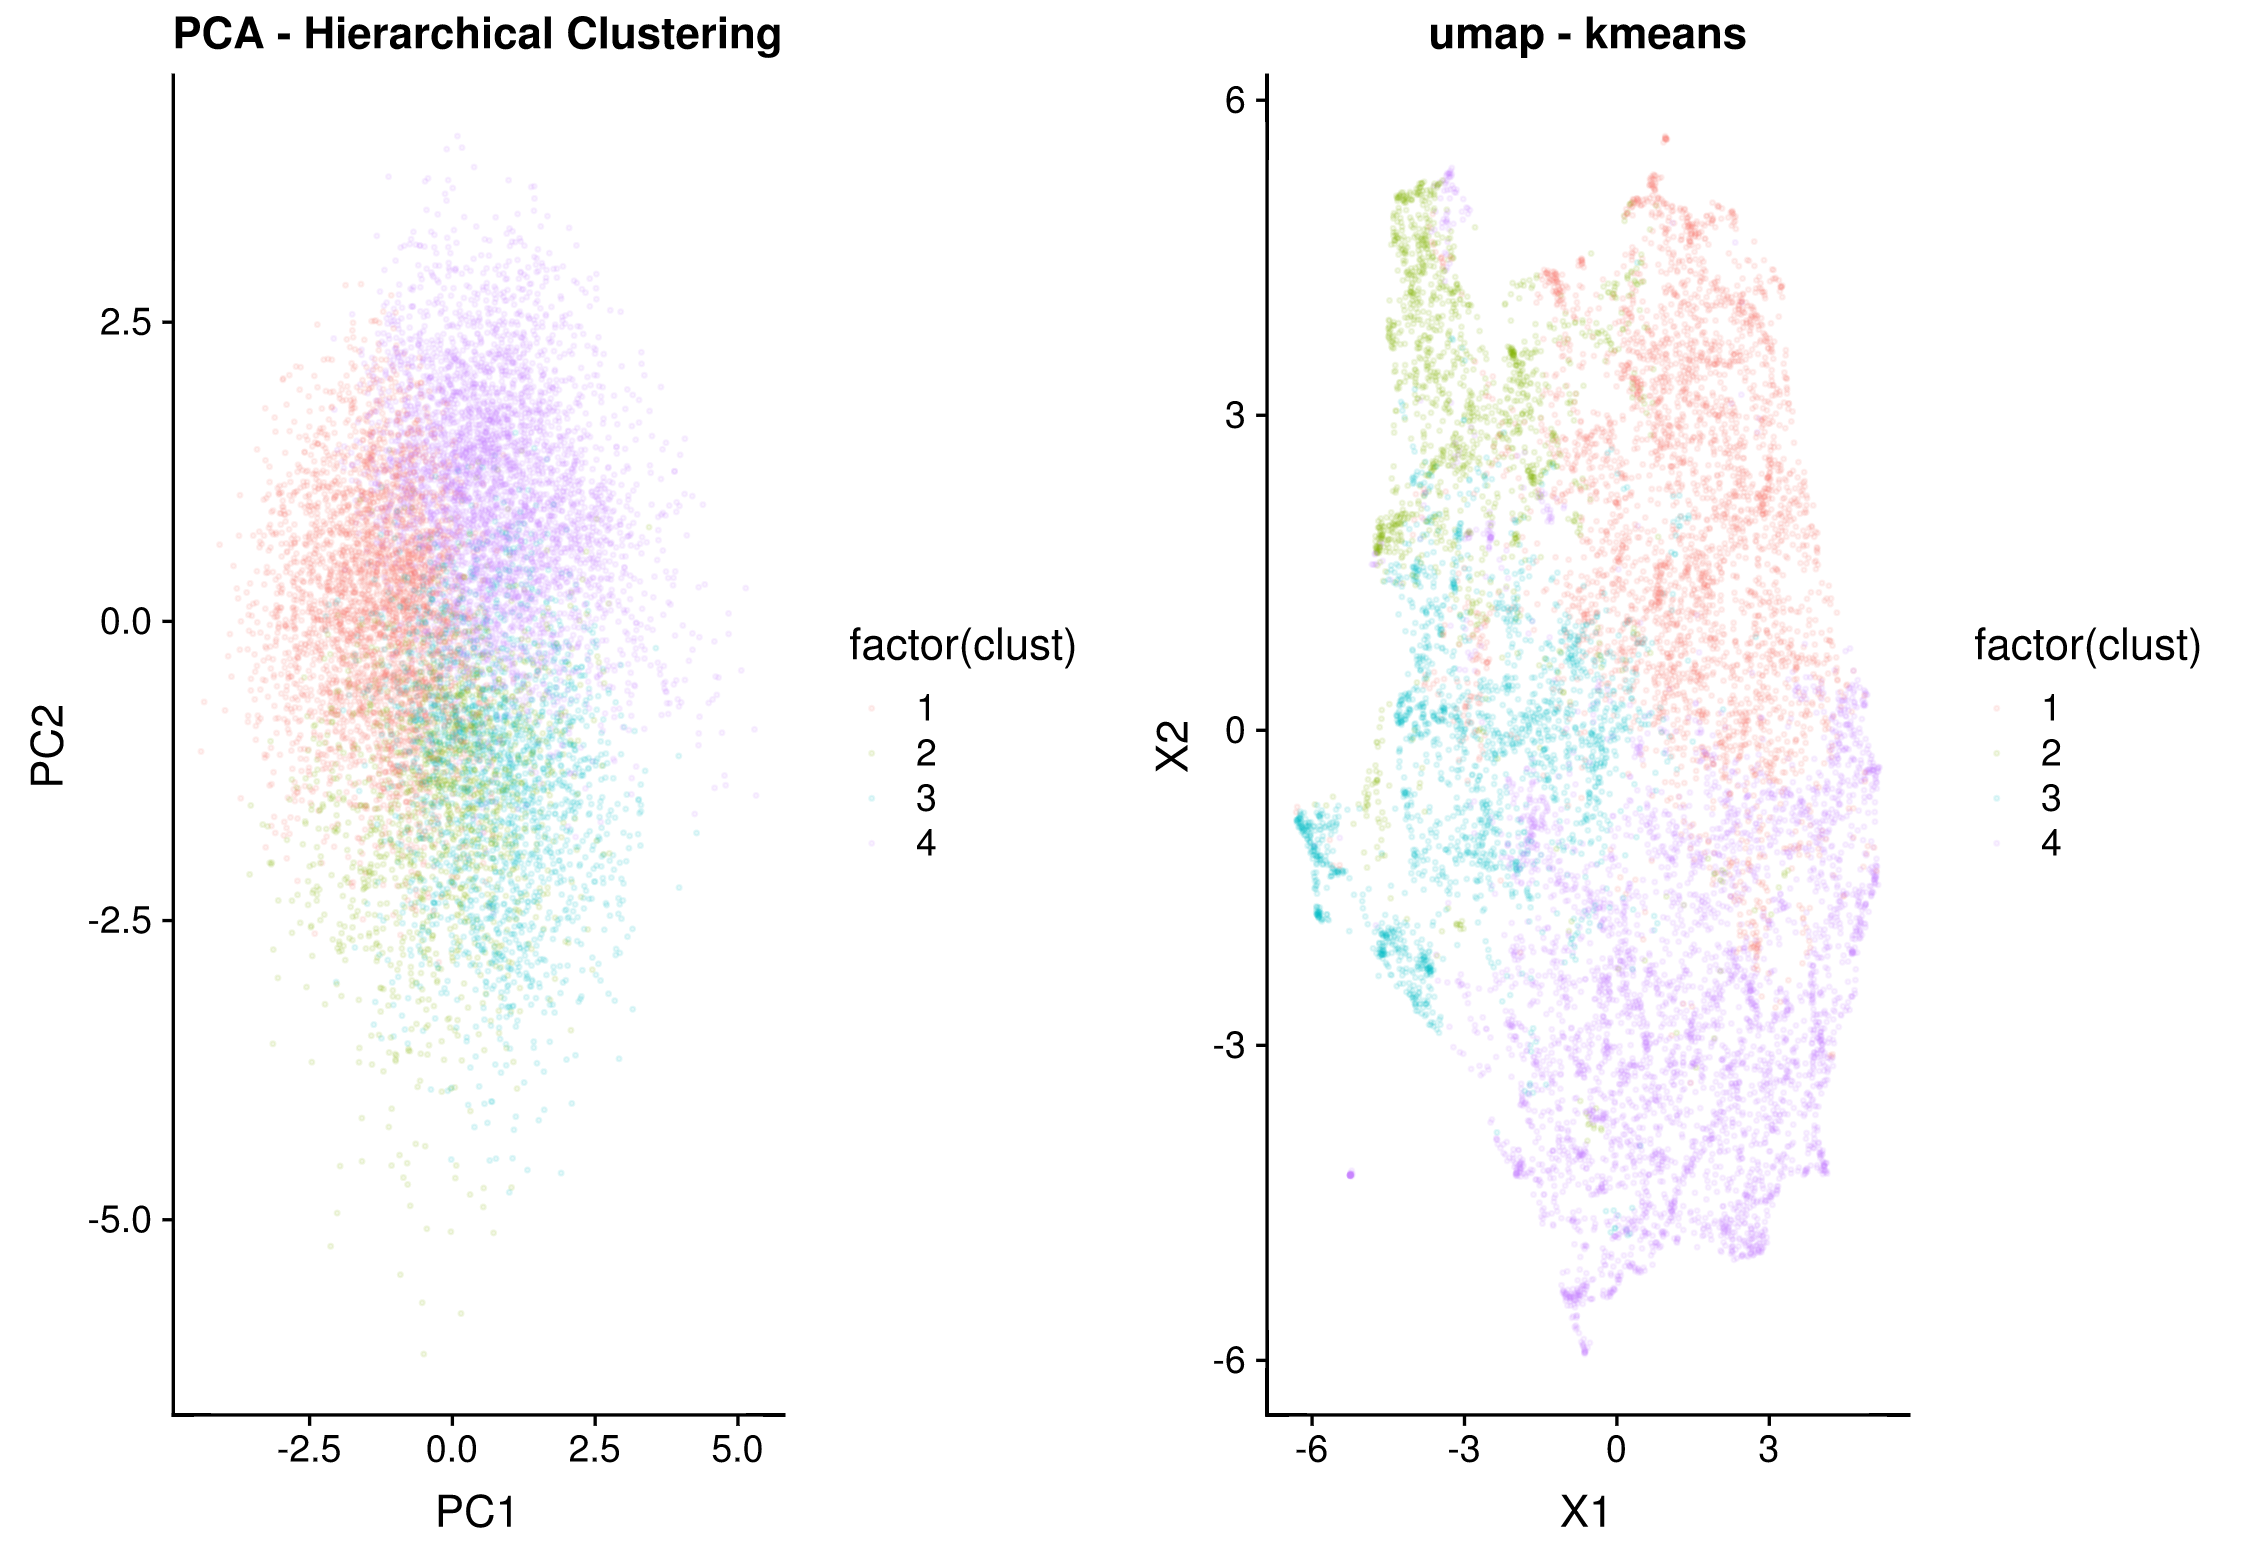
\includegraphics[scale=0.5]{fig_ACT_HC_4_Clusters.png}
  \caption{ACT clusters displayed on PCA and UMAP projections obtained using Hierarchical clustering}
  \label{fig:figHC4clusters}
\end{figure}

\section{ACT Cluster validations via patient trajectories}
\label{appendix:actpatienttrajectories}

We assessed the validity of the clusters by adding or removing features and checking individual patients’ representation and trajectory in those clusters. Figure \ref{fig:ACTclusteringAB} shows the same patient trajectory for clustering with feature selection A and clustering with feature selection B, which includes two additional features: breath amplitude standard deviation, and rolling weekly adherence score for breath count. It is notable that once computer gaming was introduced to ACT in both cases A and B the same patient moved from cluster with “expected” breath counts per ACT to a cluster characterized by much higher breath counts. This validates that there was a change over time in the patient’s ACT pattern that could be captured. The additional breath amplitude standard deviation feature (sdBreathAmplitude) make results more explainable from a clinical point of view, as the original cluster for the patient in Clustering B was characterized by a centroid with the highest sdBreathAmplitude value. 

\begin{figure}[H]
  \centering
  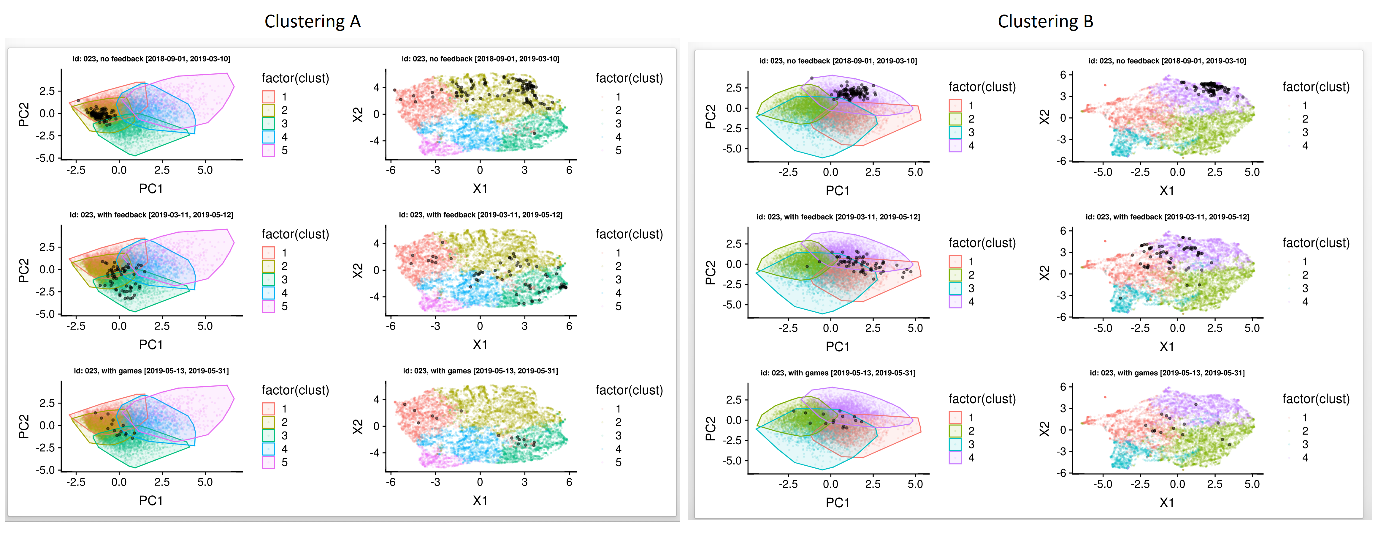
\includegraphics[]{ACTclusteringAB.png}
  \caption{Patient Trajectory on set A of features (without breath amplitude) and set B of features.}
  \label{fig:ACTclusteringAB}
\end{figure}



\section{ACT clustering with different data partitions}
\label{appendix:actdatapartitions}

We assessed the clustering stability on different data partitions. Random sampling 80~\% of the data and clustering using k-means provided very similar results with clustering on the full dataset: figure \ref{fig:ACTclusteringon80} shows that the shape of the clusters, cluster centroids as well as Silhouette Coefficients and Calinski-Harabaz Index (2200 v 1770 respectively) were comparable. 

\begin{figure}[H]
  \centering
  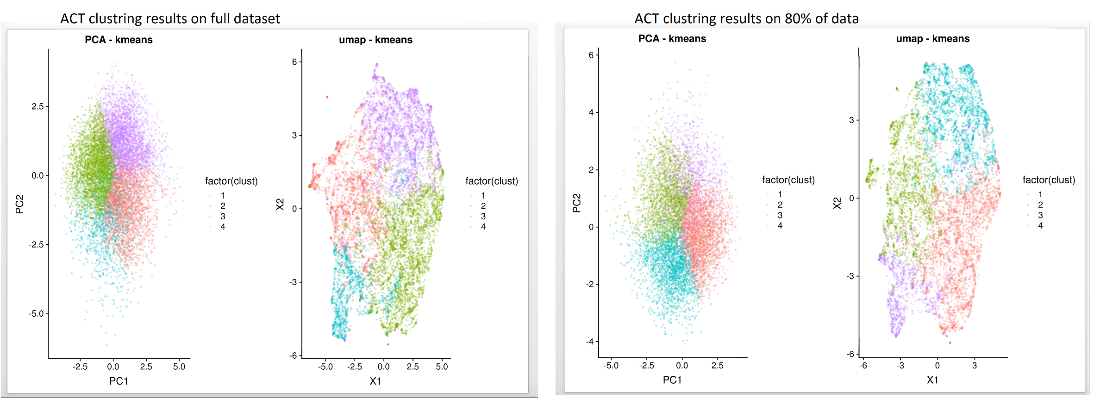
\includegraphics[]{ACTclusteringOn80.png}
  \caption{K-means clustering results on full dataset (left) and subset of data (right).}
  \label{fig:ACTclusteringon80}
\end{figure}


\end{document}